\documentclass[onecolumn, draftclsnofoot,10pt, compsoc]{IEEEtran}
\usepackage{graphicx}
\usepackage{url}
\usepackage{setspace}

\usepackage{geometry}
\usepackage{mathtools}
\usepackage{graphicx}
\usepackage{epstopdf}
\usepackage{float}
\usepackage{longtable}

\geometry{textheight=9.5in, textwidth=7in}
\geometry{margin=0.75in}

% 1. Fill in these details
\def \CapstoneTeamName{		Team TriTone}
\def \CapstoneTeamNumber{		45}
\def \GroupMemberOne{			Aidan O'Malley}
\def \GroupMemberTwo{			Christopher Hebert}
\def \GroupMemberThree{			}
\def \CapstoneProjectName{		Music Theory Application}
\def \CapstoneSponsorPerson{		Lukas Hein}

% 2. Uncomment the appropriate line below so that the document type works
\def \DocType{		%Problem Statement
                %Requirements Document
                %Technology Review
                %Design Document
                Progress Report
                }
            
\newcommand{\NameSigPair}[1]{\par
\makebox[2.75in][r]{#1} \hfil 	\makebox[3.25in]{\makebox[2.25in]{\hrulefill} \hfill		\makebox[.75in]{\hrulefill}}
\par\vspace{-12pt} \textit{\tiny\noindent
\makebox[2.75in]{} \hfil		\makebox[3.25in]{\makebox[2.25in][r]{Signature} \hfill	\makebox[.75in][r]{Date}}}}
% 3. If the document is not to be signed, uncomment the RENEWcommand below
%\renewcommand{\NameSigPair}[1]{#1}

%%%%%%%%%%%%%%%%%%%%%%%%%%%%%%%%%%%%%%%
\begin{document}
\begin{titlepage}
    \pagenumbering{gobble}
    \begin{singlespace}
        % 
\includegraphics[height=4cm]{coe_v_spot1}
        \hfill 
        % 4. If you have a logo, use this includegraphics command to put it on the coversheet.
        %\includegraphics[height=4cm]{CompanyLogo}   
        \par\vspace{.2in}
        \centering
        \scshape{
            \huge CS Capstone \DocType \par
            {\large\today}\par
            \vspace{.5in}
            \textbf{\Huge\CapstoneProjectName}\par
            \vfill
            % {\large Prepared for}\par
            % \Huge \CapstoneSponsorCompany\par
            % \vspace{5pt}
            {\Large\NameSigPair{\CapstoneSponsorPerson}\par}
            {\large Prepared by }\par
            Group\CapstoneTeamNumber\par
            % 5. comment out the line below this one if you do not wish to name your team
            \CapstoneTeamName\par 
            \vspace{5pt}
            {\Large
                \NameSigPair{\GroupMemberOne}\par
                \NameSigPair{\GroupMemberTwo}\par
            }
            \vspace{20pt}
        }
        \begin{abstract}
        % 6. Fill in your abstract  
            This document is a progress report for Team TriTone containing information about what was accomplished over the first half of winter term.
            There is a recap of the project as well as a summary individual progress, problems encountered, solutions, and where the project is headed from here.
        \end{abstract}     
    \end{singlespace}
\end{titlepage}
\newpage
\pagenumbering{arabic}
% \tableofcontents
% 7. uncomment this (if applicable). Consider adding a page break.
%\listoffigures
%\listoftables
% \clearpage

% 8. now you write!
\section{Project Recap}

The tentatively named Music Theory App is an iPhone and Android app aimed at teaching beginning composers the fundamentals of music theory in such a way that they can immediately apply the concepts toward creating their own music. 
The app presents the vision of music theory belonging to Lukas Hein, our client which he calls the schedule of tonal gravity. 
It provides a simple foundation for choosing which chords resolve to each other using a tool known as the circle of fifths.

The main page of the Music Theory App is an interactive circle of fifths.

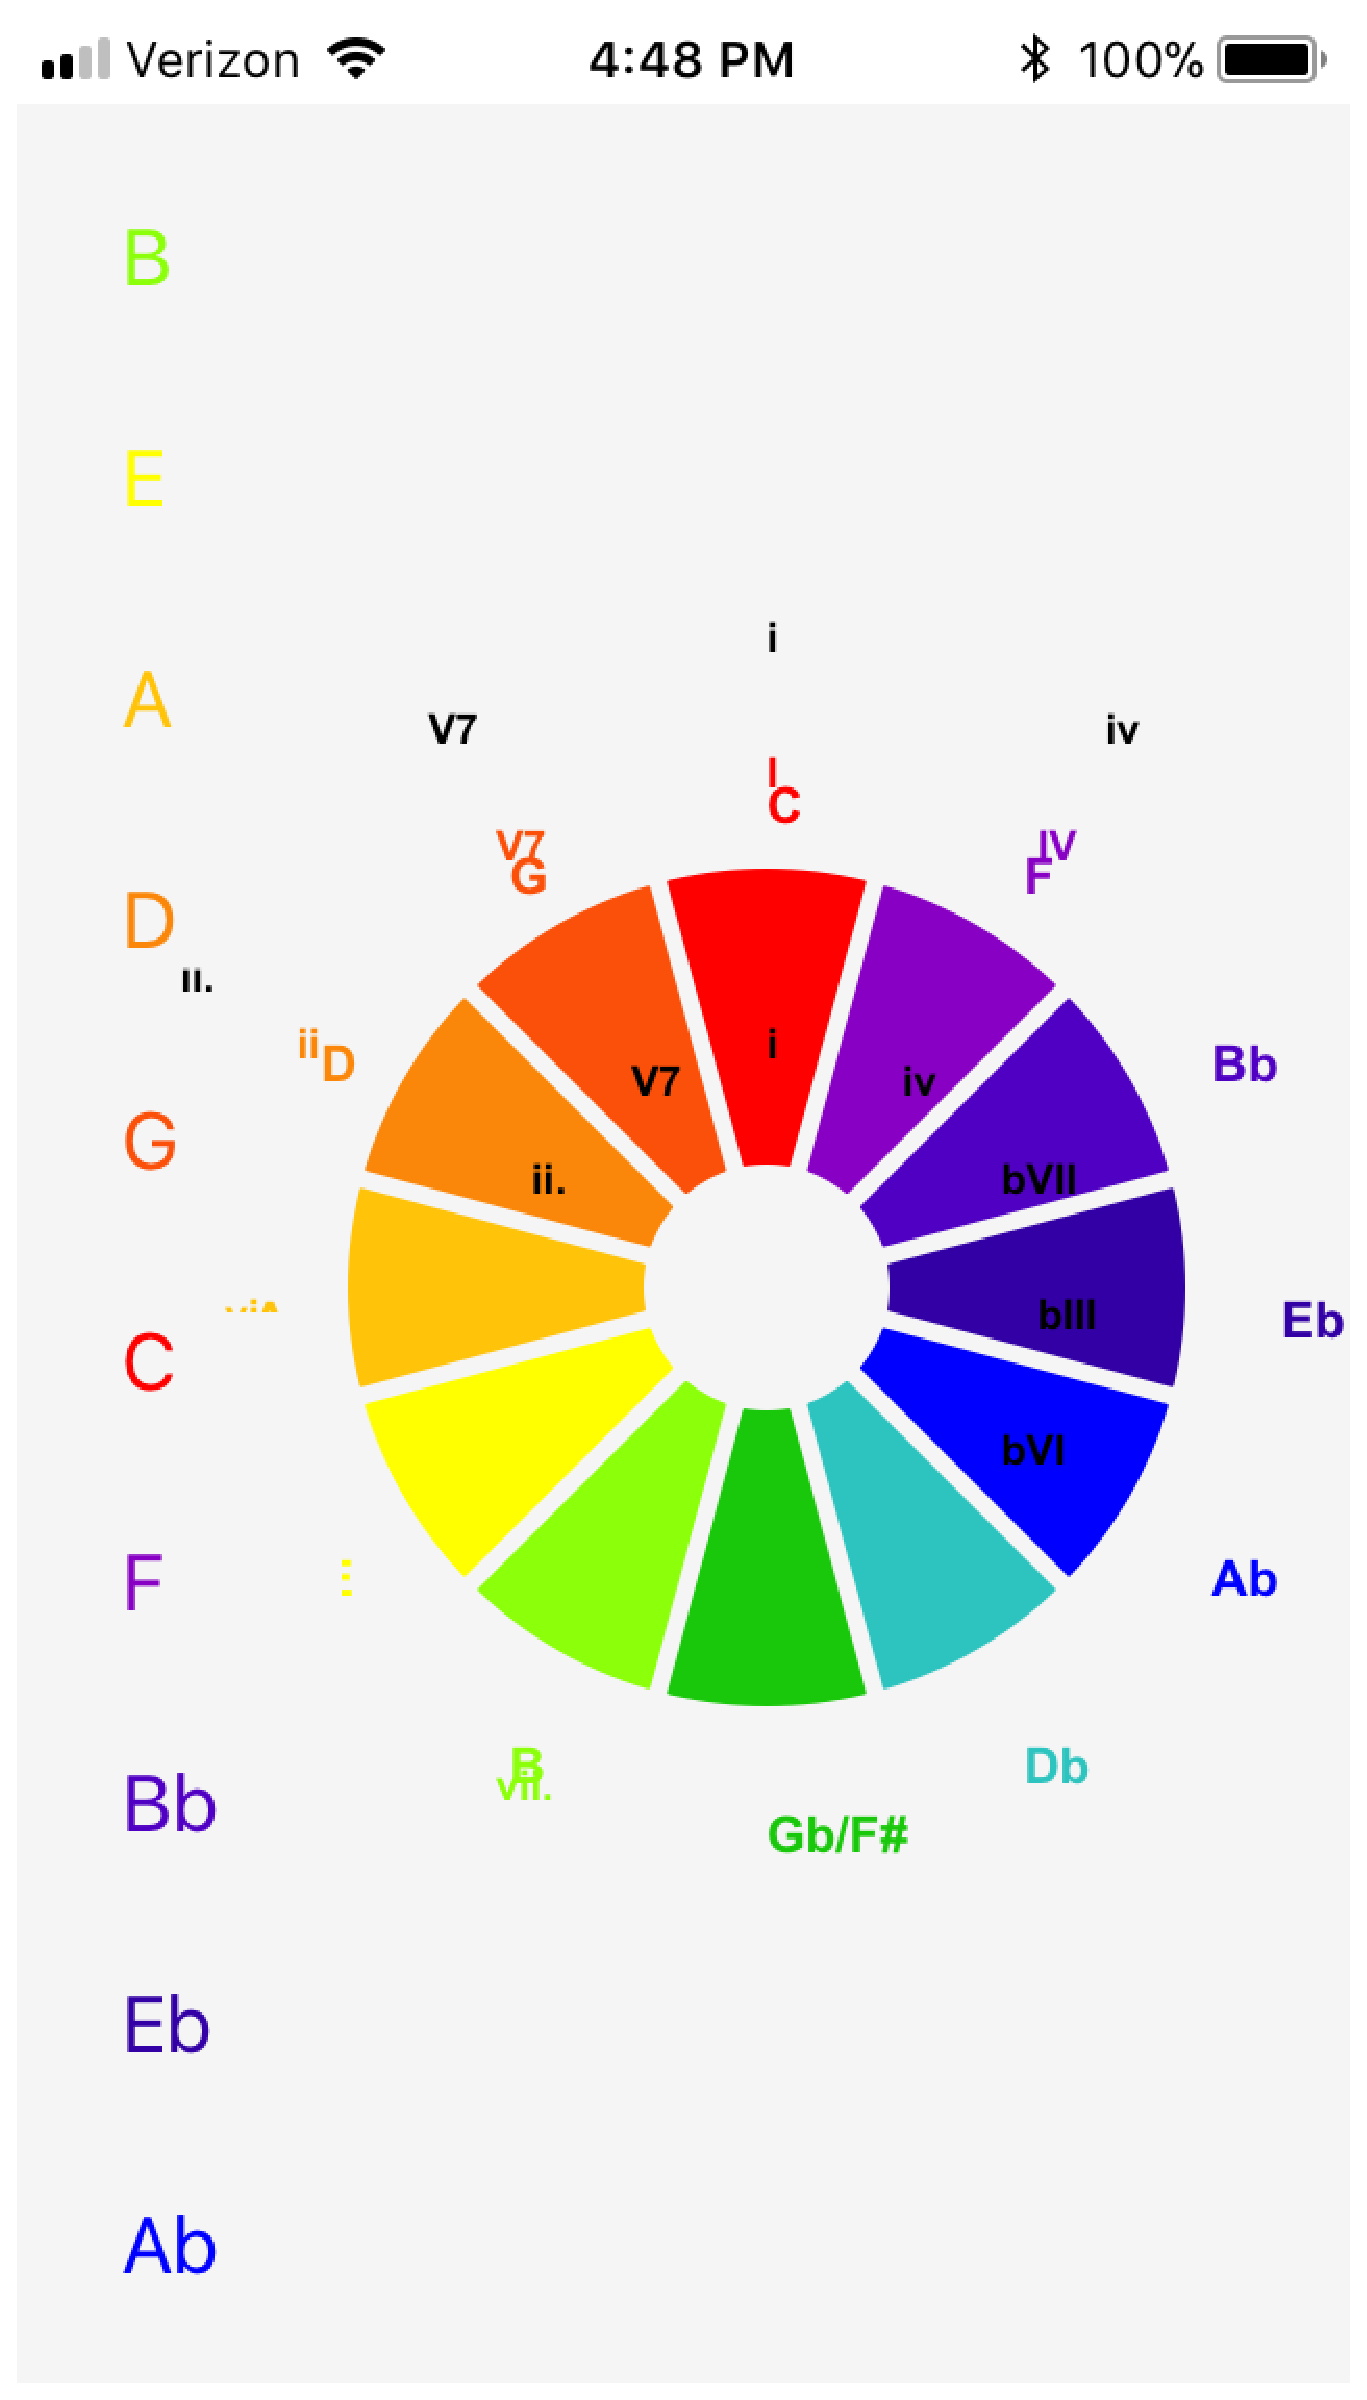
\includegraphics[width=0.25\textwidth]{cof}

The app also provides reference pages, for learning the fundamentals: including information about notes, intervals, keys, chords, and how to use the circle of fifths and tonal gravity to compose.
The app gives the musician a composition page that allows her to try composing phrases digitally, and have the app analyze the phrase according to tonal gravity theory.

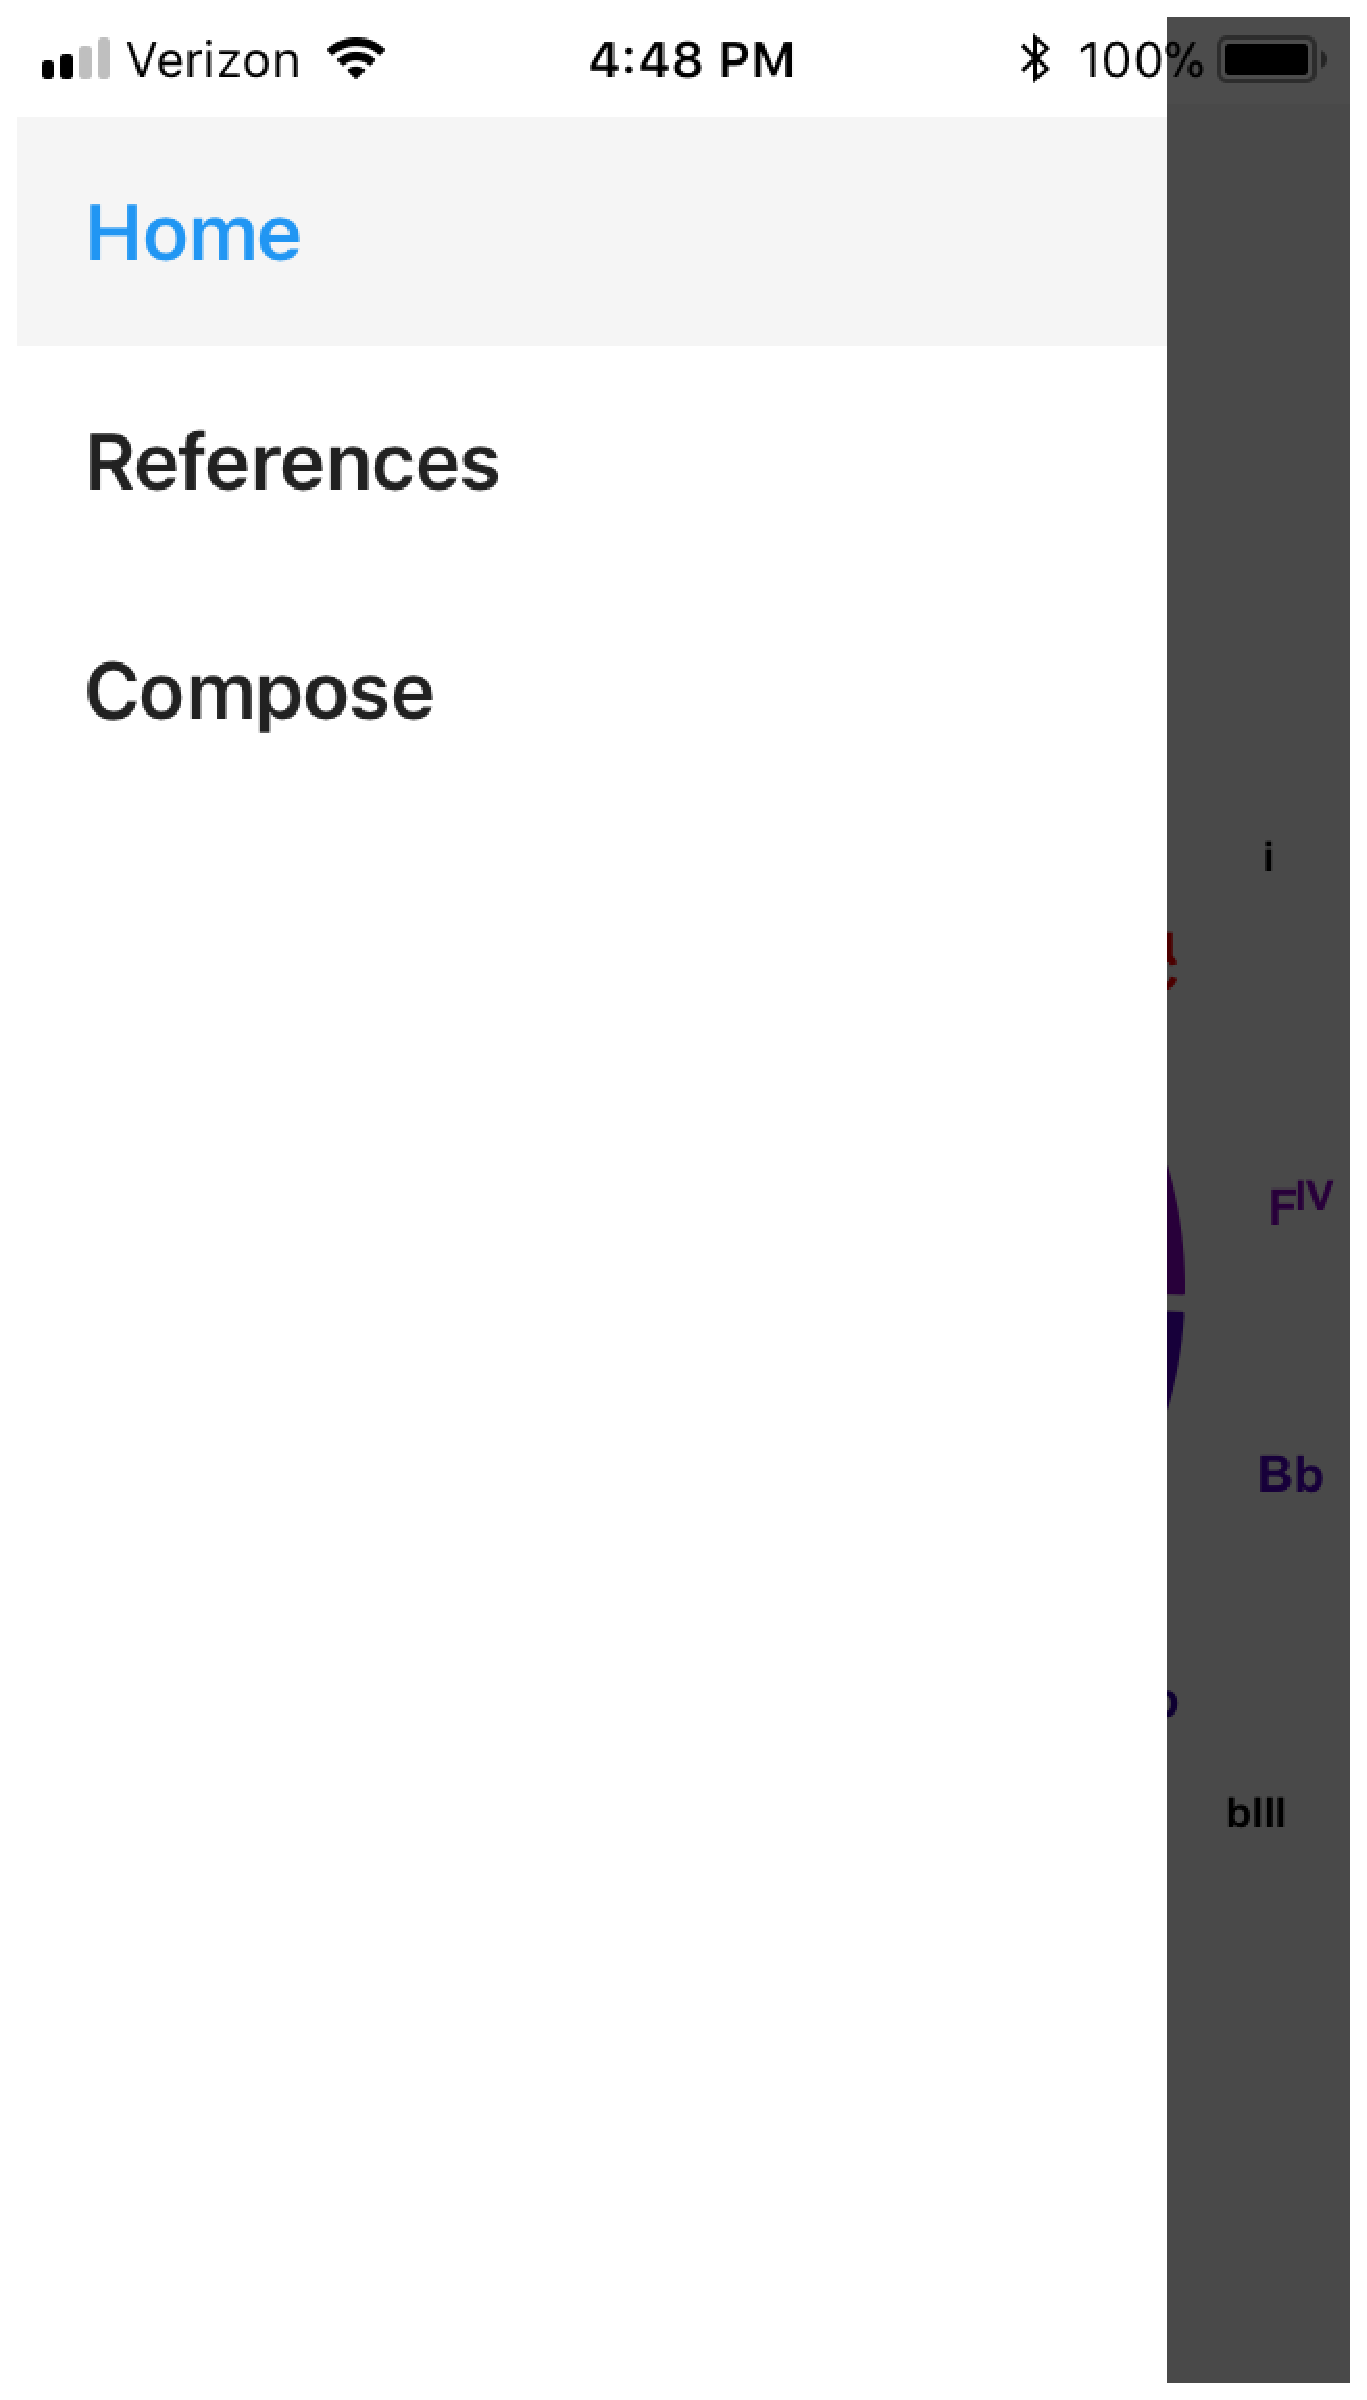
\includegraphics[width=0.25\textwidth]{menu}

\section{Aidan}
\subsection{Circle of Fifth's Restructuring}
Over winter break my focus was on the circle of fifths. 
I am actually still working on the circle of fifths, however, there have been many iterations for me to get to the point I am currently at which will be explained. 
The main issue I have faced while coding this segment of the application is really deciding on a solid structure for the code. 
For the prototype I made in fall term, all of the code was essentially in one file. 
This was mostly just because I wanted to quickly make something for Lukas so that we could come up with the design iteratively. 
However, once the true development began, I made the mistake of attempting to just add to the initial prototype file. 
This mistake was something I realized at the beginning of winter term.

The React development framework has a pretty set in stone way of coding software. 
The main idea behind React is that you split segments of the app logically into components. 
For example the Circle of Fifths page can be its own component and the Composition/Analysis page can be its own compoent. 
My mistake was thinking that I was done with components at that point (one component per screen). 
Something like the reference page for diatonic substitutions could have all of the related code in one component because it is a static file. 
However, the interactions that we need to make available on the Circle of Fifths page makes its design a different story. 
First off, the pie chart needs to be created on the screen which is its own function. 
The gesture handler also needs to get set up at some point so that the user is able to rotate the circle. 
All of the different notes and qualities for the current key needs to be surrounding the circle. 
The sidebar needs to be functional and interactive. 
The user needs to be able to change the key and have all of the details on the screen reflect those changes immediately. 
I could go on and on about all of the functionality of this screen, however, the main takeaway is that the code needed to be split up more from what I had at the prototype stage. 
The next step was to decide how to go about splitting up the screen into multiple components.

Before beginning to think about the different components that will make up the Circle of Fifths screen, however, there was another feature of React and of application development in general that needed to be figured out: how to handle application state. 
In React, each component has its own state object and when fields within this object are updated, the render function of the component is triggered to run again to show any changes that have occured on the screen. 
This was how I was handling state initially; everything was in the same component so everything could use the same state which was really easy. 
But now I needed to split up the code into components and to handle state in this new situation, I had two options. 
The first option was to use props capabilities of React. 
The second option was using Redux. Props in React are really similar to using component state described earlier. 
When a component is defined with the html syntax in the JSX language, the component can also have additional fields. 
These fields are similar to how html elements can have additional fields such as “class” or “value” on an input element. 
When a component is defined like this, the values of these fields are passed down to this component in the props object. 
For example, if a component called Circle was defined as follows in the render function of a container component: a Circle component with a radius of 3, then when the developer is in the code of the Circle component, they could reference the value of radius by calling ``this.props.radius''. 
There is another way of handling state between multiple components that also uses props, however, which brings in another library called Redux.

Redux works by having a global state object that is accessible to any component in a project.
What a developer has to do to use this global state is to use the connect function of the “react-redux” npm package and define what fields should be taken from the Redux state to return a component that has a connected redux state. 
However, the Redux state has to be set up first to be able to use components with connected state. 
Redux works by using actions and reducers to set up its state object. 
Actions are plain text that describe an action that the developer wants to happen in the application. 
For example, if a user wanted to change the current key on the Circle of Fifths screen, we could create a redux action called ``CHANGEKEY''. 
When an action is “dispatched”, the reducer comes into play. 
When a user invokes a gesture that should change the key, this ``CHANGEKEY'' action is dispatched to the redux reducer in the code. 
The reducer contains the initial state of this segment of the application and it also has definitions for what should happen to the state when specific actions are dispatched. 
For example, the reducer for the Circle of Fifths segment of the app would define a way of altering the state when the ``CHANGEKEY'' action is dispatched to it. 
Most likely, the reducer would want to return the initial state with the value of the current key equal to the definition of the new key belonging to the action. 
I found the idea of Redux to be really easy to wrap my head around compared to the other manner of handling state with props. 
The simplicity of the state of Redux was attractive enough to me to use it for the Circle of Fifths screen to avoid the more complex idea (in my eyes) of continually passing props downwards between components.

Now that I have decided on a way of structuring the components in the Circle of Fifths page (see image below) and since I have decided on a way of handling the Circle of Fifths applications state with Redux, I will be able to finish up this segment of the application and have it tested by the end of this term. 
It was a struggle figuring out all of the interactions a user needed and to also learn Redux, however, I am in a very good place and the code that will result from these design decisions will be much closer to the industry standard than before.

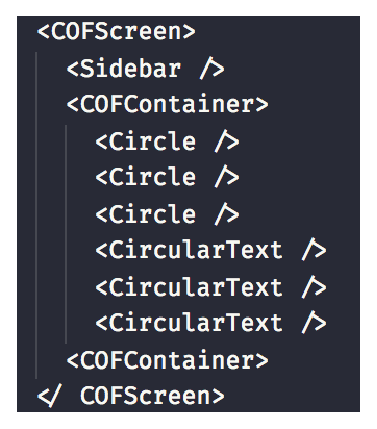
\includegraphics[width=0.25\textwidth]{cof-html}

Moving on from the Circle of Fifths screen, this term I also added a menu to the application so that a user is able to easily navigate through the many pages in the project. 
This was a pretty easy addition with the help of open source npm packages. 
We now have a functional drawer menu that is accessible on any screen by swiping right from the left side of the screen.

What I have still have left to do once I complete the Circle of Fifths screen is to figure out how to run the application on Android. 
We chose React Native because it is a cross platform development framework, however, Kazuriah was the only member of the team with an Android phone to test on. 
Now that he is no longer available, it is just another issue we have to deal with on top of losing a great group member. 
I have had trouble trying to run the application on an Android emulator on my computer so we might need to borrow an Android for a day at some point soon to start testing on those devices.
It is still not much of a worry at the moment because all of the code should translate between platforms in theory, it would just be good to have an idea of the changes that need to be made, sooner rather than later.
Lastly, testing will be another focus throughout my work this term. 
I am excited to get a release out soon after working with Lukas and Chris some more this term.


\section{Chris}
\subsection{Reference Pages}
Last quarter, we had a de facto group organization where Aidan was in charge of the Circle of Fifths page, Chris was in charge of Composition and Analysis, and Kaz was in charge of the reference pages. 
Unfortunately, this quarter our team lost Kaz. 
Fortunately, when we met with Lukas for the first time after our break, he approached us with the desire to organize the content reference pages himself. 
This meant however, that we needed to allow him to write content for the reference pages, including text, headings, pictures, gifs, and musical notation, without needing to know how to program. 

I came up with an interim, and potentially permanent, solution: Markdown. 
Markdown is a simple enough language for non-technical people to use, that gives them the ability to write HTML without needing to code or check their syntax.
Currently, Lukas is still organizing his thoughts on how to present the music theory topics succinctly.
As they are now, the Reference pages allows for Markdown text to be specified as a string with minimal escaping required in JavaScript using ES6 string templates.

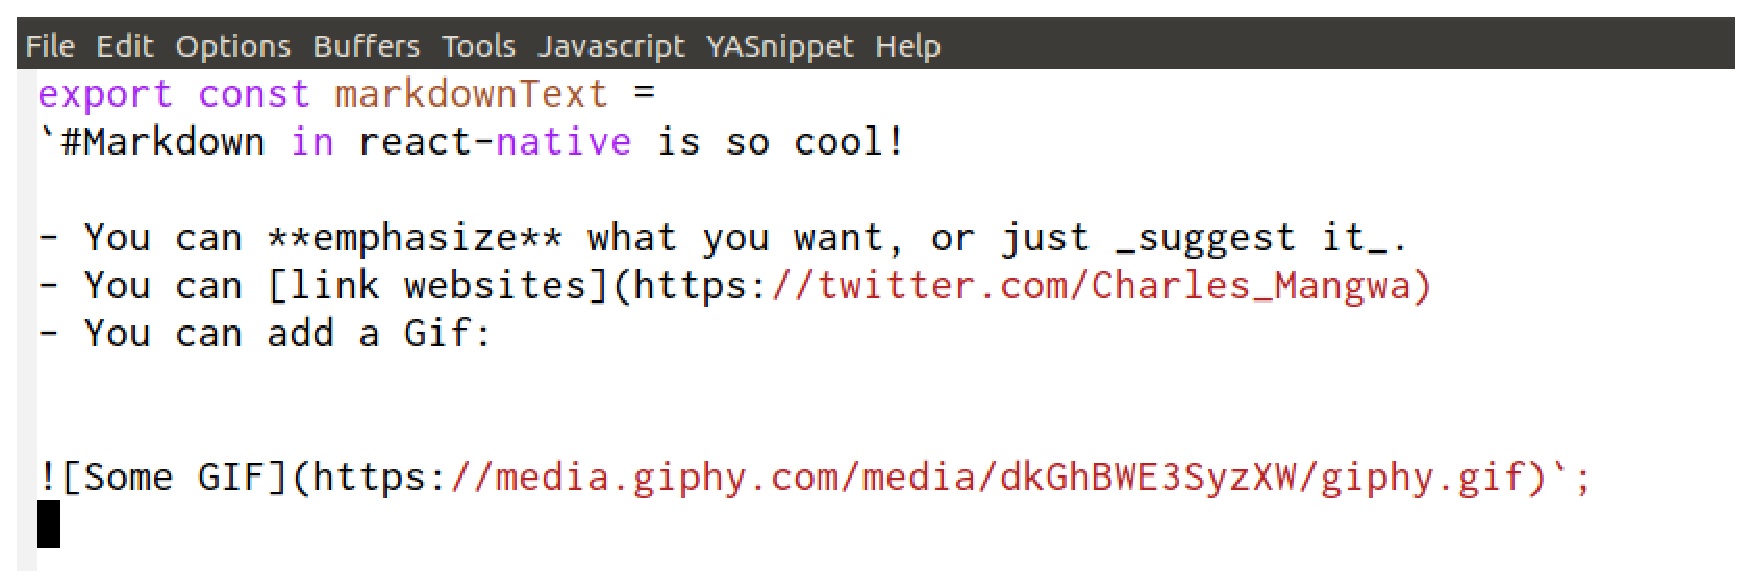
\includegraphics[width=0.75\textwidth]{markdown-code}

By using these string templates, we only need to escape backticks in the Markdown text Lukas sends us.
I chose to use the simple-markdown package on NPM in order to implement this.

Additionally, we needed a convenient way to navigate the different Reference pages. 
I chose to use a swipe view, with dots at the bottom indicating the number of pages available, and where you were in the page.

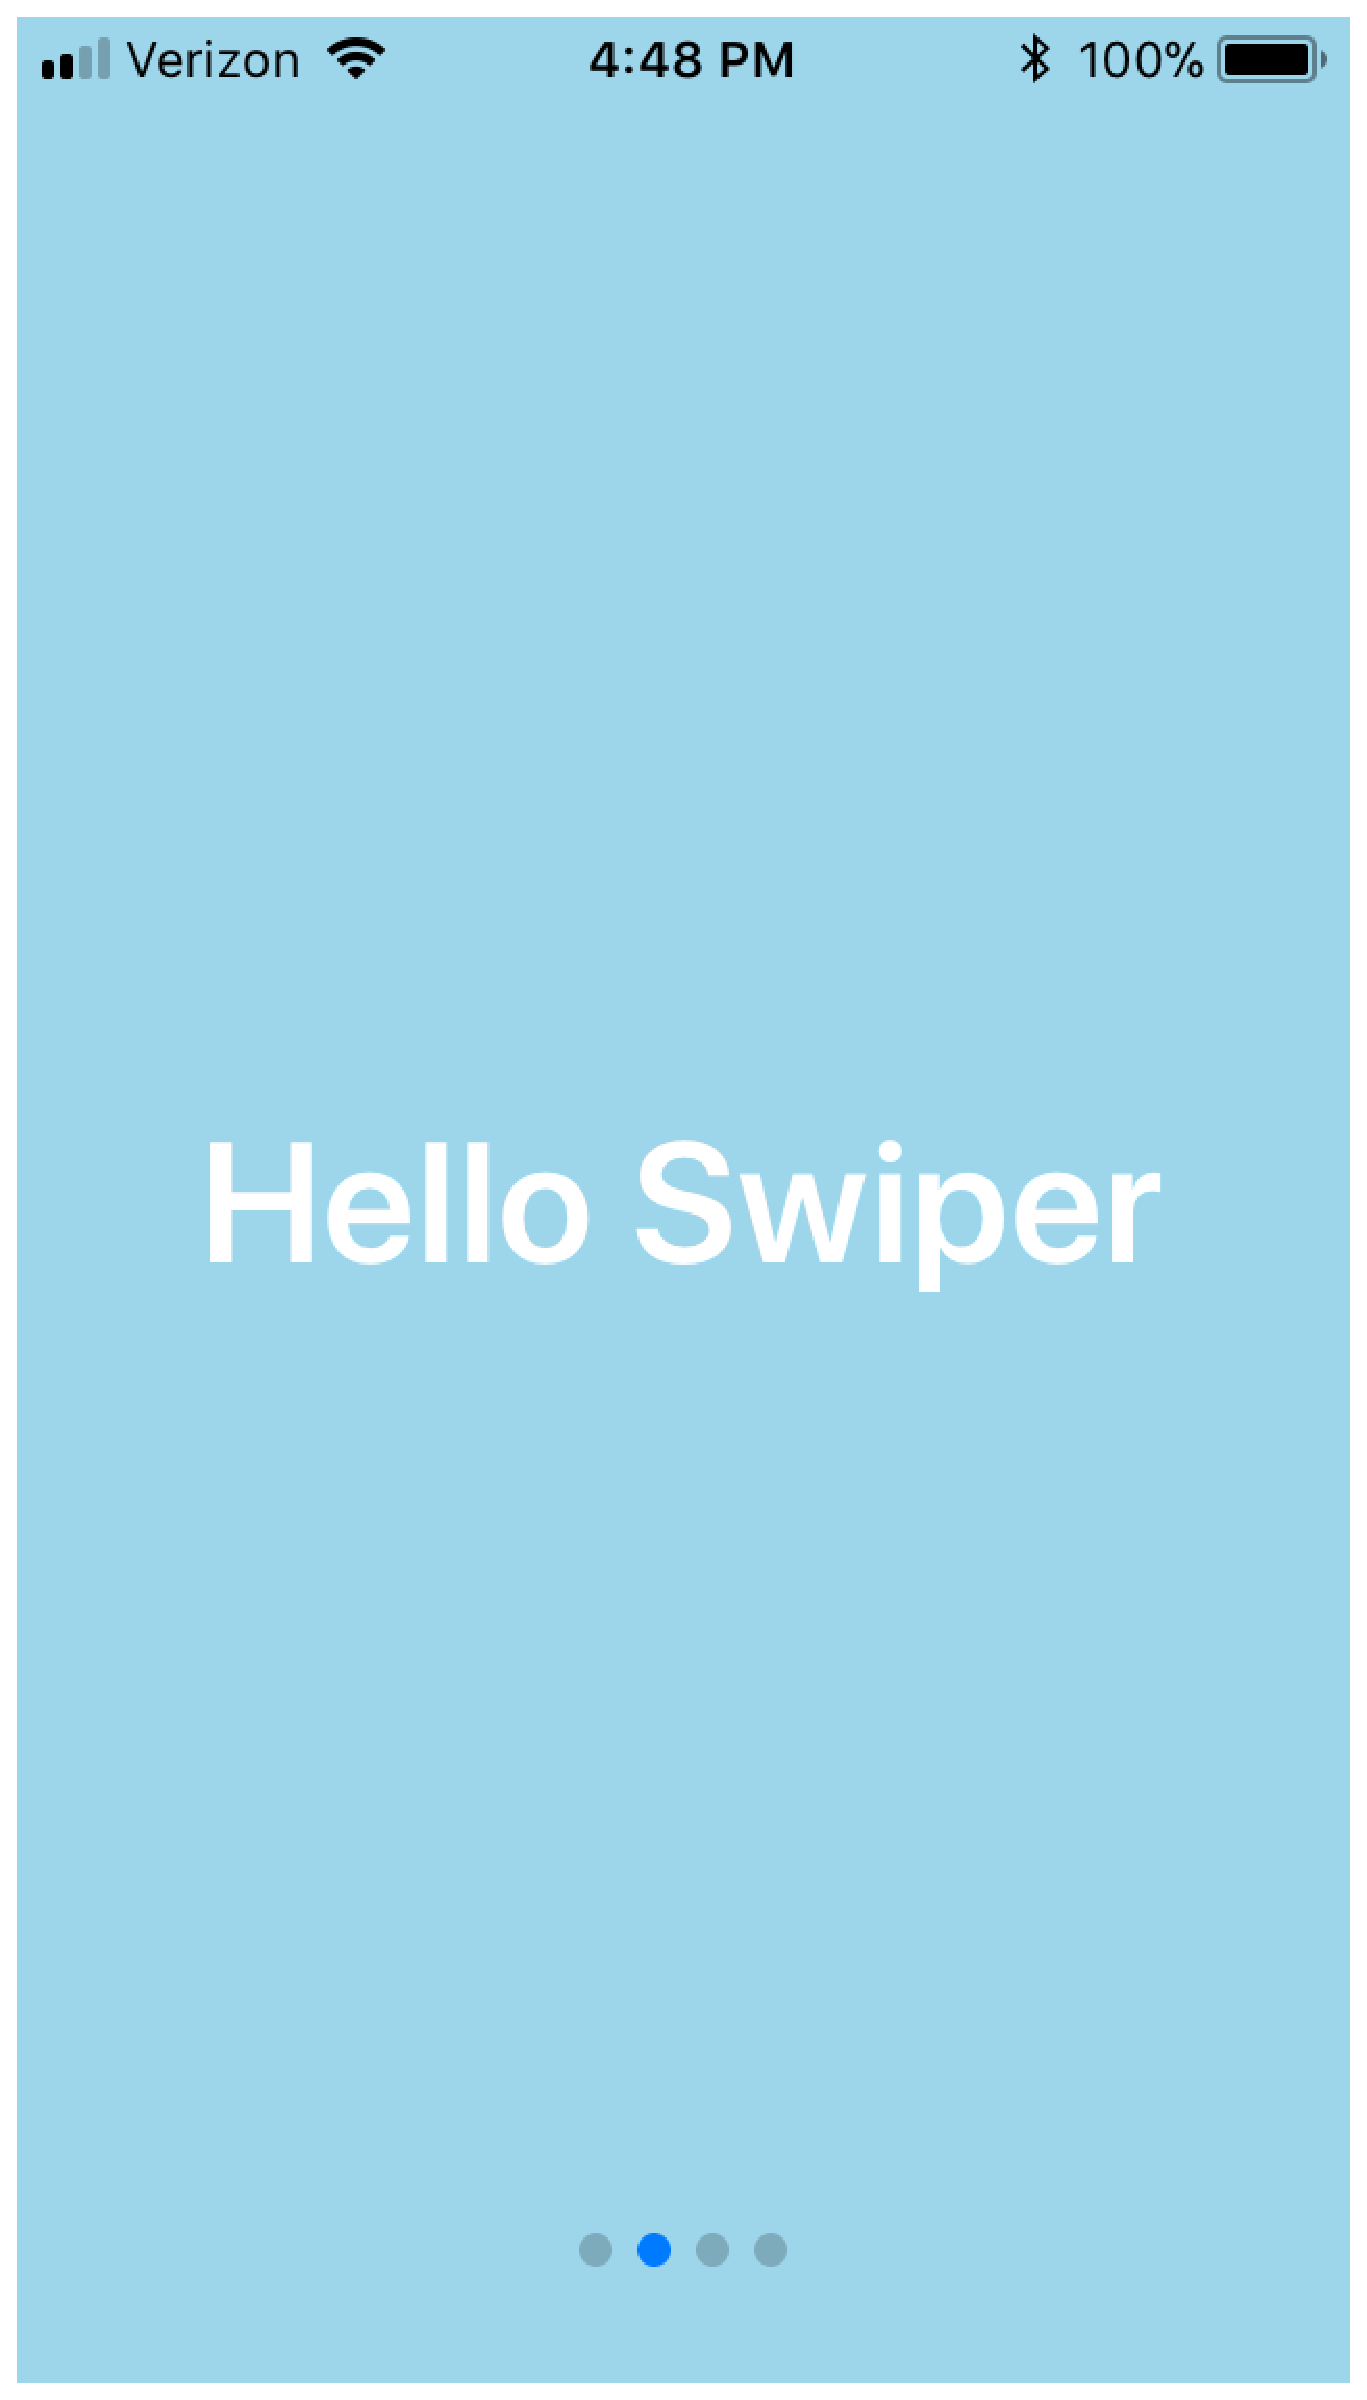
\includegraphics[width=0.25\textwidth]{swipe}

In order to finish the Reference pages, we really need Lukas to determine how the theory needs to be organized.

Lukas has mentioned that he wants to be able to write in musical notation that would look good in context.
This means we would incorporate an existing package that can draw musical notation, we could write our own simple functions and components for drawing notation, or we can use an external package to create images.

It is possible that the best way to present the material is to offer some form of interactivity.
For example, it may be best to demonstrate chords by allowing users to select chords and automatically showing the notes in the chord.
This would be an addition to the design document, but it would be a nice touch which would really help sell the app to users, investors, and expo walkers.

\subsection{Composition And Analysis Page}
The de facto organization from the beginning gave me the Composition and Analysis page.
Before making anything fancy, I did what I could to throw in what we had talked about in the design document into the app.
This meant creating a container component, based on (i.e. copied from) the Circle of Fifths page belonging to Aidan.
I ended up removing any of the code I didn’t understand, and putting in the bare minimum to make a functional composition page, so that the code ended up completely my own.

One of the first headaches I encountered was with JSX.
JSX is an extension of the JavaScript that allows HTML like language to be embedded in JavaScript code.
This makes sense when React applications are being developed, but React Native does not use HTML.
One of the main problems I encountered with this notation was that I could not comment out JSX (HTML) using JavaScript comments.

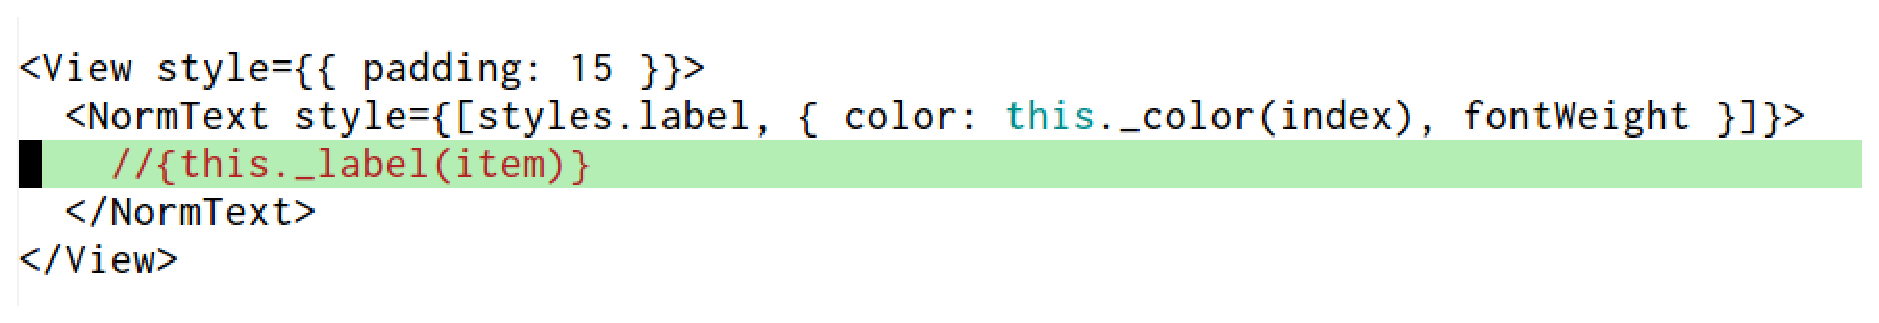
\includegraphics[width=0.75\textwidth]{jsx-comment}

This was frustrating for me to develop with, so I fortunately was able to opt out of this and use plain JavaScript function calls.
Aidan saw that I was doing it this way, and it led to a debate between us.
The main points Aidan brought up were that JSX is industry standard, and that my code is not as easy to read, and that JSX would become easier to understand over time.
We talked about this for a bit, but eventually decided to go our separate ways on the issue: Aidan would use JSX in the Circle of Fifths code he was working on, and I would not use it on the Composition or Reference pages.

Once I had dodged any problems I had with JSX, I was able to quickly throw together a Composition Page.
I used the segmented-controls package which creates radio buttons for root tones, chord qualities, and 7th qualities.
Currently the Composition page allows you to enter in a chord, which is displayed as plain text in a made up music notion.
For example, C7 is written as CMajMin.
I did this so that I could get feedback from Lukas on the interface before finishing implementation.
This turned out to be a good idea, because Lukas decided that it would be simpler to not include 7ths at all.
Instead, he decided on 4 chord qualities: major, minor, diminished, and dominant (which has a 7th in it).
In the app page I showed him it also had an augmented chord quality, but Lukas decided that this wouldn’t be appropriate for beginning music theory.
I had also stubbed out an analysis portion of the composition page.
When the user pressed the Analyze button text would appear that said something like “G to G: Invalid transition. Breaks rule 1”.

Lukas wanted two things different.
He wanted an Analyze toggle that would automatically analyze the composition when enabled.
He also wanted to move away from language like “breaking rules” and rather just describe what the transition is in terms of the Tonal Gravity theory.
He wanted us to use the following (valid) movements: step up, leap up, step down.
He wanted us to distinguish these from the invalid movements: leap down, parallel motion.

Right now, the Composition page still uses the old qualities (including Augmented) and 7th qualities, and the analysis button.


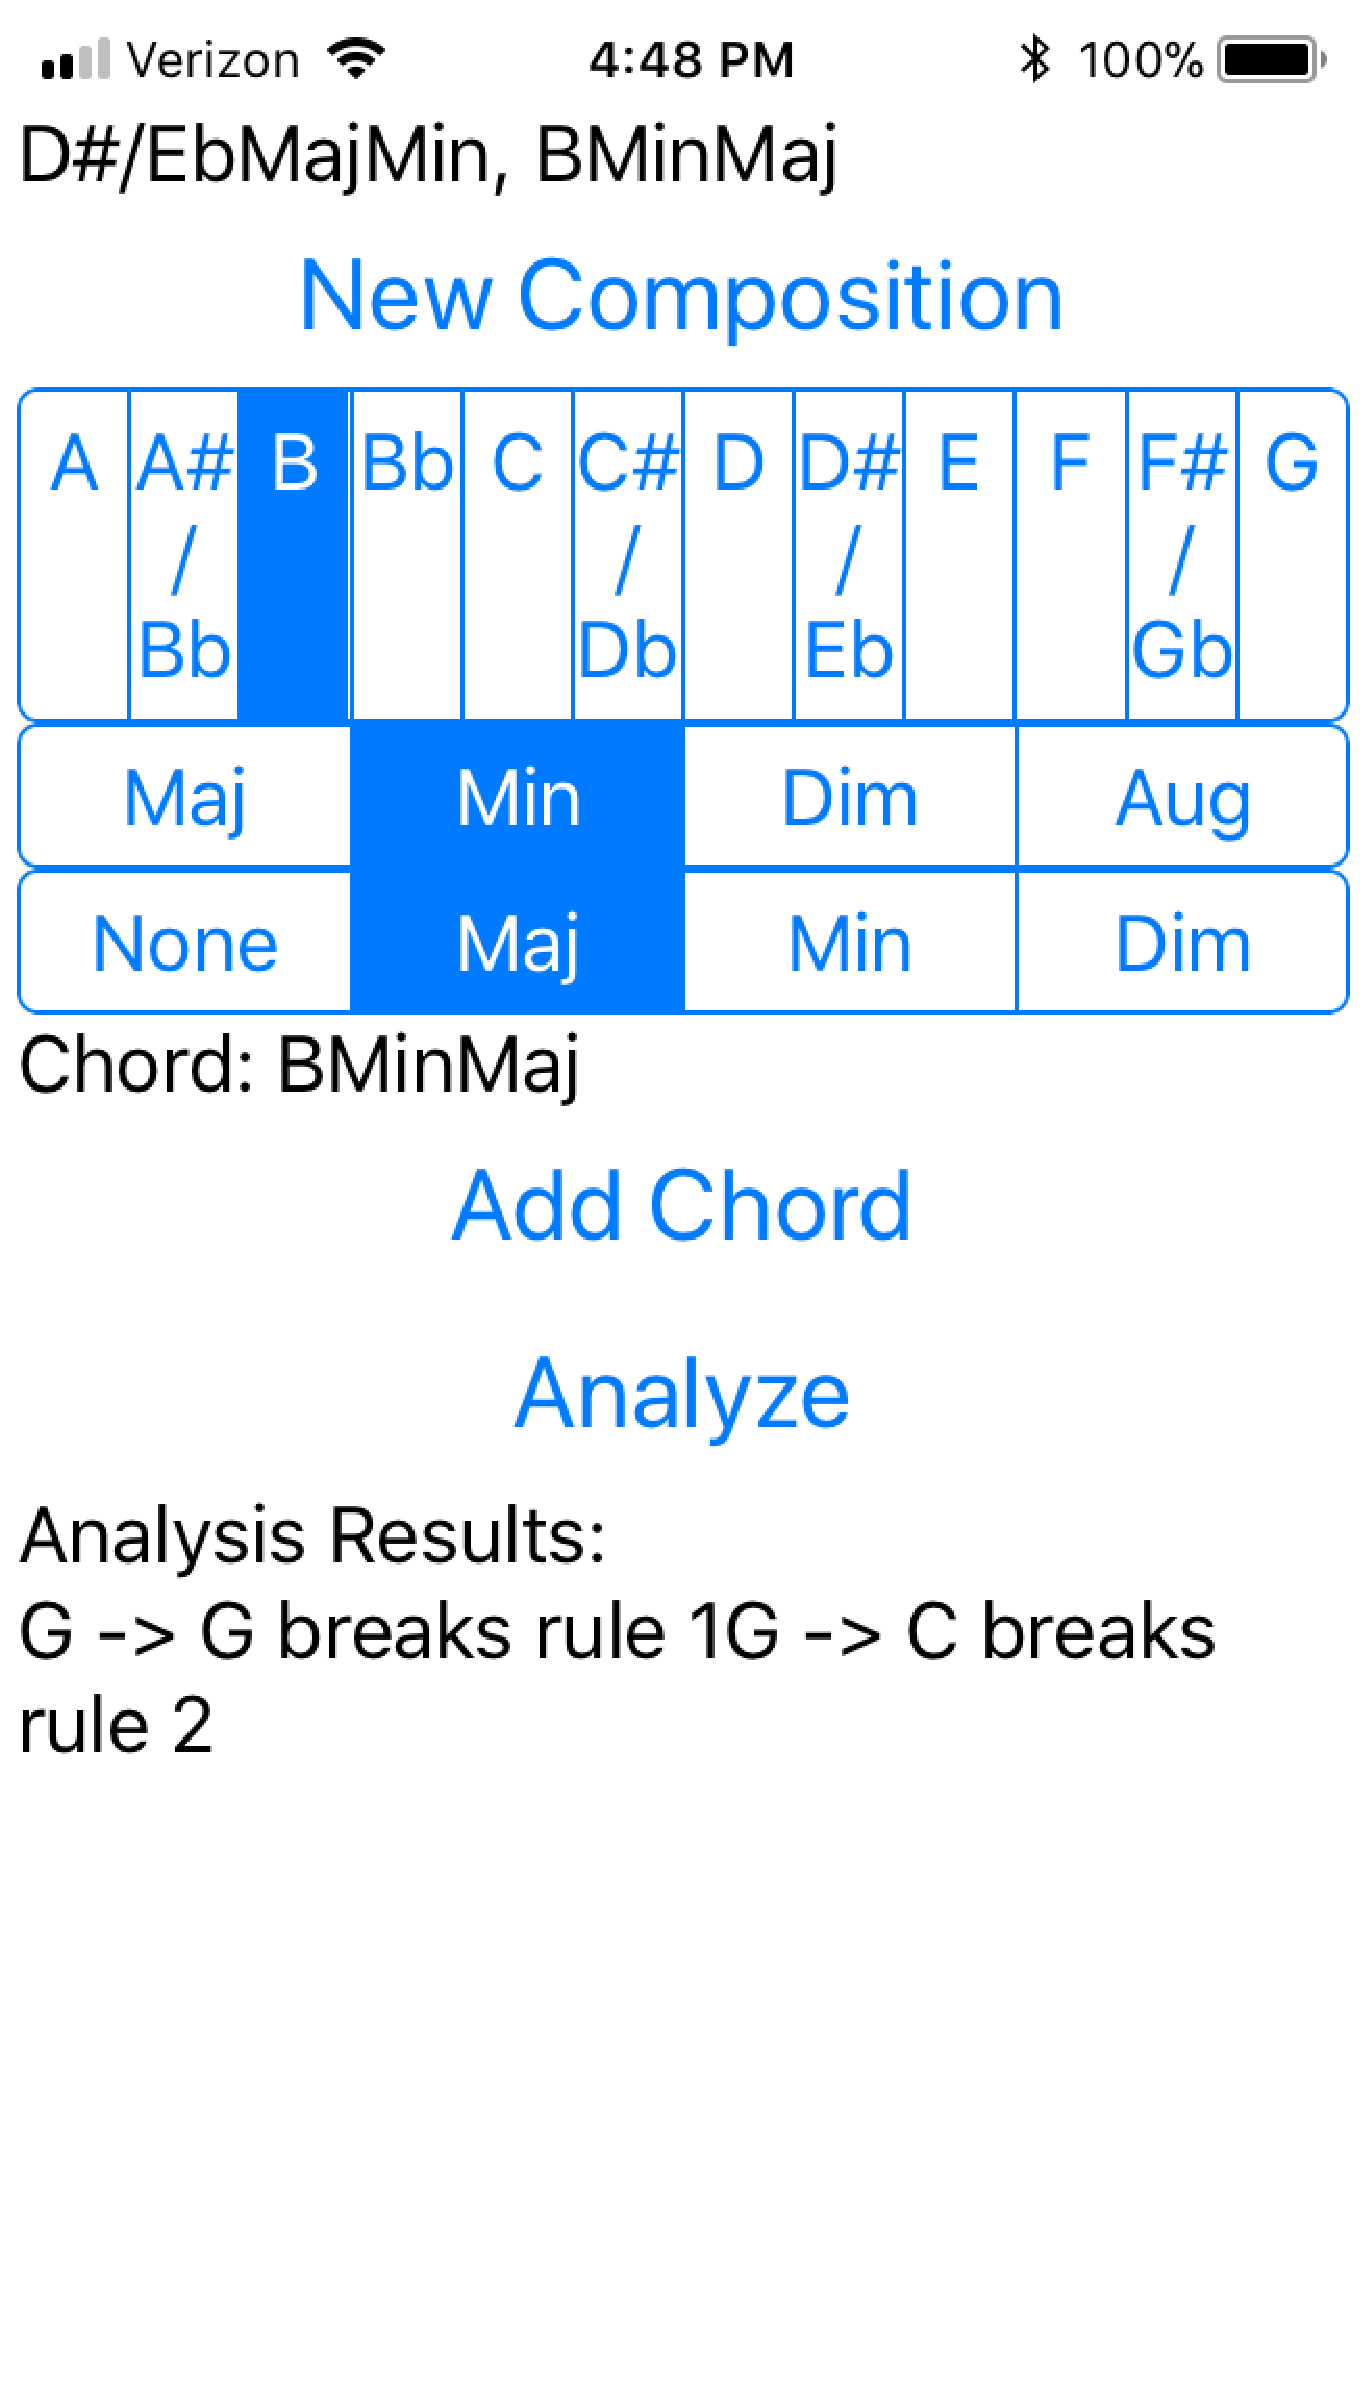
\includegraphics[width=0.25\textwidth]{compose}

Going forward, we will be implementing Lukas’ suggestions for automatic analysis, and chord qualities.
We will revise our design document as needed.

\section{Conclusion}
We feel very good about our progress.
We have a clear goal of what we need to do next.
We have a solid team balance, even though we lost Kaz.
We have a friendly working relationship with our client, Lukas, and will continue to meet with him weekly.
Moving forward, we will need to look at getting an Android device, working on our poster, and our sales pitch.

\end{document}
